\documentclass[conference]{IEEEtran}
% \IEEEoverridecommandlockouts
% The preceding line is only needed to identify funding in the first footnote. If that is unneeded, please comment it out.
\usepackage{amsmath,amssymb,amsfonts}
\usepackage{algorithmic}
\usepackage{graphicx}
\usepackage{textcomp}
\usepackage{xcolor}
\usepackage[style=ieee, autocite=inline]{biblatex}
\addbibresource{ZoteroLibrary.bib}
\begin{document}

\title{Discrete-time Control Contraction Metrics (DCCM) for Quasistatic Planar Pushing using Smoothed Dynamics\\
{\footnotesize MIT 2.152[J] Nonlinear Control Project Report}
}

\author{\IEEEauthorblockN{Shao Yuan Chew Chia}
\IEEEauthorblockA{
\textit{Harvard University}\\
Cambridge, MA \\
shaoyuan\_chewchia@college.harvard.edu
}}

\maketitle

\begin{abstract}

\end{abstract}

\section{Introduction}
% Why control through contact is difficult - non smooth dynamics
Planning and control through contact is an important task in Robotics. Robots interacting with the environment need to make and break contact in order to complete tasks but this has proved challenging due to the non-smooth nature of contact dynamics. This has traditionally been done using hybrid planners and controllers with guards and resets where different dynamics are considered based on enumerated contact modes. An alternative approach has been proposed in \autocite{pangGlobalPlanningContactRich2023} where contact dynamics are smoothed to create more informative gradients in global planning of contact-rich manipulation tasks. In this paper we apply these same smoothing techniques to explore the controllers that this enables.

% Why control through contact is difficult - underactuated
Another way in which control through contact is difficult is that these systems are highly underactuated. The state of the unactuated objects cannot be controlled directly.

% Current methods for control through contact

% Why we would want to use Control Contraction Metrics

% CCMs for underactuated systems
This work builds on \autocite{manchesterUnifyingRobotTrajectory2018} which demonstrates the effectiveness of CCMs on cannonical underactuated systems such as Cart-Pole.

% CCMs for discrete time
as well as \autocite{weiControlContractionMetric2021} that extends work in \autocite{manchesterControlContractionMetrics2017} to discrete time.

\section{Preliminaries and Problem Formulation}
\subsection{Quasistatic Assumptions}
We will assume that our system is quasistatic, meaning at each time step velocities and accelerations of the system are 0. This corresponds to having a high amount of damping and is a reasonable assumption in the 2D planar pushing setup where we restrict pushing velocities to be low and there is a large amount of friction between the object and table surface. As a result, the state of our system only consists of positions.

\subsection{Analytically Smoothed Contact Dynamics}
In this work we use the analytically smoothed contact dynamics and corresponding simulator developed by \autocite{pangGlobalPlanningContactRich2023}. Contact dynamics are formulated as an unconstrained convex program where the contact and friction contraints are moved into the objective function using a log barrier function. The effect of this is that there is a log barrier penalty for violating the contact constraints. Constraints can exert force even if they are not active and this translates to producing a force at a distance.

We plot the force at a distance effect of the smoothed contact dynamics in Figure \ref{fig:smoothed_contact_dynamics}. We see that for a high weight, which corresponds to a small force at a distance, the next $b_x$ is close to 0, but as the log barrier weight decreases, the box is pushed further to the right.

% Figure showing force at a distance
\begin{figure}[t]
	\centering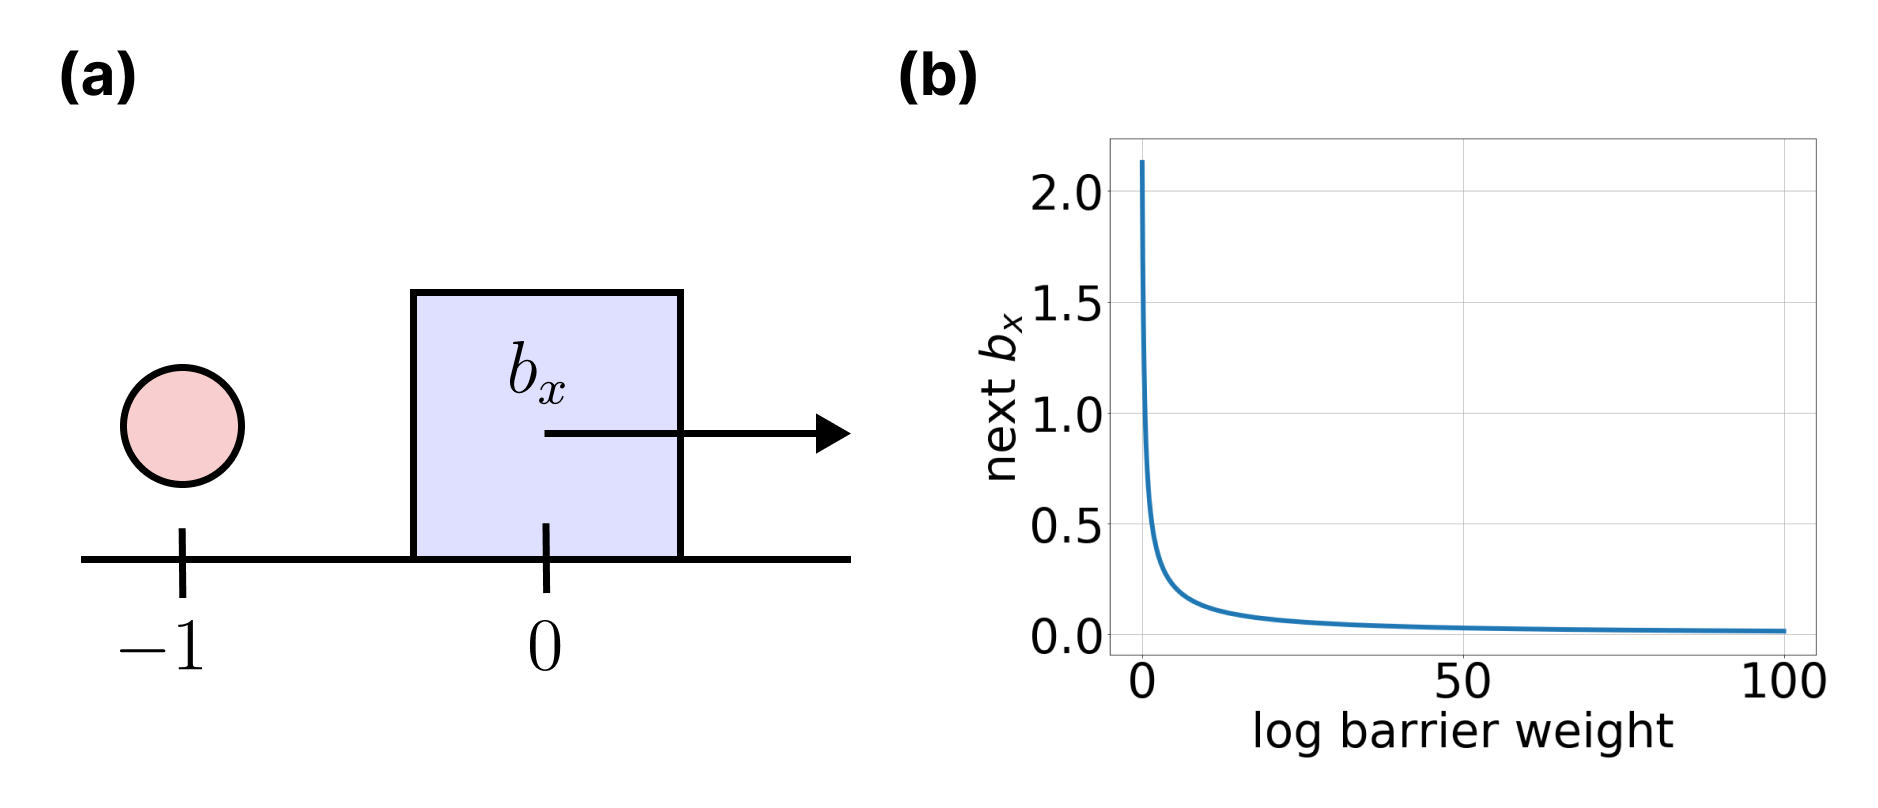
\includegraphics[width = 0.45 \textwidth]
	{figures/smoothed_contact_dynamics.png}
    \caption{Force at a distance effect of smoothed contact dynamics. (\textbf{a}) A system consisting of an actuated point finger at $x=-1$ and unactuated box at $x=0$, (\textbf{b}) The next $b_x$ after rolling out one step of the analytically smoothed dynamics with different log barrier weights.}
	\label{fig:smoothed_contact_dynamics}
	\vskip -0.25 true in
\end{figure}

\subsection{Planar Pushing System}
The state of 
\begin{equation}
    x = \begin{bmatrix}b_x & b_y & b_{\theta}& s_x& s_y\end{bmatrix}^\top
\end{equation}

control input $u$ are absolute position commands for the sphere
\begin{equation}
    u = \begin{bmatrix}u_x\\ u_y \end{bmatrix}
\end{equation}

The system evolves in nonlinearly in discrete time and is control affine. The dynamics are defined as

\begin{equation}
    x_{k+1} = f(x_k) + g(x_k)u_k
\end{equation}

where $f$ and $g$ are smooth functions due to the smoothing of the contact dynamics described in the previous section.

The differential dynamics are defined as
\begin{equation}
    \delta_{x_k} = A(x_k)\delta_{x_k} + B(x_k)\delta_{u_k}
\end{equation}
where $A(x_k) = \frac{\partial (f(x_k) + g(x_k)u_k)}{\partial x_k} \in \mathbb{R}^{5 \times 5}$ and $B(x_k) = \frac{\partial (f(x_k) + g(x_k)u_k)}{\partial u_k} \in \mathbb{R}^{5 \times 2}$ are the Jacobians of the dynamics.

We can define the state feedback control law
\begin{equation}
    \delta_{u_k} = K(x_k)\delta_{x_k}
\end{equation}
where $K$ is the state dependent feedback gain matrix.

Generalized infinitesimal squared distance in the positive definite metric $M$ is denoted $V_k$
\begin{equation}
    V_k = \delta^\top_{x_k} M_{k} \delta_{x_k}
\end{equation}

And by substituting the differential dynamics and control law, we can see that the generalized infinitesimal squared distance at the next time step is

\begin{equation}
	\begin{aligned}
	V_{k+1} & = \delta^\top_{x_{k+1}} M_{k+1} \delta_{x_{k+1}} \\
	& = \delta^\top_{x_k} (A_k + B_k K_k)^\top M_{k+1} (A_k + B_k K_k)\delta_{x_k}
	\end{aligned}
\end{equation}

The contraction condition can then be expressed as
\begin{equation}
	V_{k+1} - V_k \leq 
	- \beta V_k <
	0
\end{equation}

which simplifies to
\begin{equation}
	\label{eq:contraction_condition}
	(A_k + B_k K_k)^\top M_{k+1} (A_k + B_k K_k) - (1 - \beta) M_k < 0
\end{equation}

\autocite{weiControlContractionMetric2021} showed that equation \ref{eq:contraction_condition} can be transformed via Schur's complement (among other transformations) into
% Create a 2x2 matrix
\begin{equation}
	\label{eq:contraction_condition_schur}
	\begin{bmatrix}
		W_{k+1} & A_k + B_k L_k \\
		(A_k + B_k L_k)^\top & (1 - \beta) W_k
	\end{bmatrix} > 0
\end{equation}
where $W := M^{-1}$ and $L := KW$

\section{Methods}
\subsection{Contraction Metric and Controller Synthesis}
\subsubsection{Sum of Squares (SOS) Programming}
In order to synthesize the contraction metric and controller, we use the SOS programming framework described in \autocite{weiControlContractionMetric2021} with some slight modifications.

\begin{equation}
	\begin{aligned}
	\min_{l_c, w_c, r} & r \\
	s.t. & \forall k, w^\top \Omega w - r w^\top w \in \Sigma(x_k, u_k, w) \\
	& r \geq 0.1
	\end{aligned}
\end{equation}

where $\Sigma(x_k, u_k, w)$ is the set of SOS polynomials that satisfy the contraction condition in equation \ref{eq:contraction_condition_schur}. $l_c$ are the polynomial coefficients of $L$ and $w_c$ are the polynomial coefficients of $W$.
\begin{equation} 
	\begin{aligned}
	\Omega &=
	\begin{bmatrix}
		W_{k+1} & A_k + B_k L_k \\
		(A_k + B_k L_k)^\top & (1 - \beta) W_k
	\end{bmatrix} \\
	% W_k is a 5x5 symmetric matrix
	W_k &= 
	\begin{bmatrix}
		W_{11_k} & W_{12_k} & W_{13_k} & W_{14_k} & W_{15_k} \\
		W_{12_k} & W_{22_k} & W_{23_k} & W_{24_k} & W_{25_k} \\
		W_{13_k} & W_{23_k} & W_{33_k} & W_{34_k} & W_{35_k} \\
		W_{14_k} & W_{24_k} & W_{34_k} & W_{44_k} & W_{45_k} \\
		W_{15_k} & W_{25_k} & W_{35_k} & W_{45_k} & W_{55_k} \\
	\end{bmatrix} \\
	% L_k is a 2x5 matrix
	L_k &=
	\begin{bmatrix}
		L_{11_k} & L_{12_k} & L_{13_k} & L_{14_k} & L_{15_k} \\
		L_{21_k} & L_{22_k} & L_{23_k} & L_{24_k} & L_{25_k} \\
	\end{bmatrix} \\
	\end{aligned}
\end{equation}

each $W.._{k} = w.._c v(x_k)$ is a polynomial constructed from the row vector of coefficients of $w.._c$ and the monomial basis vector $v(x_k)$. For example, if the degree of the polynomial is chosen to be $4$,
\begin{equation}
	v(x_k) = [x^4_{k_4}, x_{k_3}x^3_{k_4}, x^2_{k_3}x^2_{k_4}, \cdots ,x_{k_1}, x_{k_0}, 1]
\end{equation}
where $v(x_k)$ has $126$ elements. $L.._k = l.._c v(x_k)$ is similarly defined.

We note the difference in the way we use the slack variable $r$ compared to \autocite{weiControlContractionMetric2021}. In \autocite{weiControlContractionMetric2021}, the constraints on the optimization program are $w^\top \Omega w - r I \in \Sigma(x_k, u_k, w), r \geq 0$. In practice we found that in some cases, especially when generating a higher degree metric, that the solver would return a trivial solution where $r$, $w_c$ and $l_c$ are extremely small numbers (on the order of $1e-17$). By setting a higher bound on $r$, we force the solver to find a solution where the contraction condition is satisfied with a greater buffer and the returned coefficients of $w_c$ and $l_c$ are larger.

Another difference is that we do not have closed form equations for the $A$ and $B$ matrices whihc would allow us to enforce the contraction conditions over all states. Instead, we sample a set of state, control action pairs and enforce the contraction condition over these samples. Since $M$ is smooth, we can expect the contraction condition to be satisfied over at least a small local region around each sample. However, if the samples are too sparse, the contraction condition may not be satisfied over all the states around the desired trajectory.

We solve this SOS program using Drake's Mathematical Program \autocite{DrakeModelBasedDesign}, which uses Mosek under the hood to solve this Semidefinite Program (SDP).

\subsubsection{Sampling Strategy}
To get a contraction metric valid over the entire state space we would have to densely sample the entire state space. However, the available RAM on the machine sets an upper bound of the size of the optmization program, which for a monomial basis of degree $4$, was around $2000$ samples. Thus, to get a contraction metric and controller that had good performance at least in the vicinity of the desired trajectory, we only sampled states and control actions from a small region around the desired trajectory. This is a clear limitation of the current approach and future work would involve finding a way to enforce the contraction condition over a larger portion of state space.

\subsection{Online Geodesic and Controller Computation}

\section{Results and Discussion}

\subsection{Degree of metric on}
Higher degree means its more able to find a contraction metric for a system with more "warped" dynamics, i.e. if there is less smoothing. 

But higher degree also means less samples can be used, and increased computation time.
\subsection{Effect of number of samples on controller performance}

\printbibliography

\end{document}
